\chapter{Introduction}\label{chapter:intro}
\lhead{\emph{Introduction}}
Our picture of the cosmos in the 21$^{\rm st}$ century appears to have dissolved into a vista of almost paralysing darkness and confusion. Headlines proclaim that physicists do not understand 95\% of the contents of the Universe. While in essence they might be right, we can safely assert that the statistical error on this ignorance is a very small value indeed. The Universe, we know, is hiding from us a pair of mysterious entities. The challenge faced by modern science is how best to baptise these shadowed creatures in the purifying light of human understanding. Of the two, the most recently emerged, dark energy, remains tantalisingly out of reach. The other, dark matter, is a paradox; elusive yet ubiquitous, strange and exotic, yet apparently essential for the Universe to function as we know it, and for us to exist.

The beginning of the dark matter (DM) story is often attributed to the work of Zwicky in the 1930s~\cite{Zwicky:1933gu} from whom originates the moniker ``dunkle materie''. Since then dark matter has developed into one of the central unsolved problems in the collective mind of the physics community. Given such intense focus and the now overwhelming compendium of evidence for the presence of a large quantity of invisible matter, it is all the more surprising then that from the perspective of particle physics the nature of that matter remains as elusive as ever. The 21$^{\rm st}$ century has brought about the advent of precision cosmology. With it, compelling and near-conclusive evidence for a primarily dark contribution to the energy density of the Universe. The hope is that the efforts of particle physics experiments and observations can rise to the task of exposing the identity of dark matter. Just as the evidence from galactic rotation curves began a revolution in the understanding of galaxies, we too expect the unmasking of dark matter to reveal a new realm of particle physics. Indeed dark matter and the questions it asks of us have inspired the construction of some of the most sensitive and complex machines ever conceived. It is perhaps grandiose, but not overly optimistic to claim that the first detection of interacting dark matter will merely be the prelude to a new era of physics.

In this introductory chapter we present a bird's eye view of the evidence for dark matter (Sec.~\ref{sec:intro_evidence}), candidates from particle physics (Sec.~\ref{sec:intro_candidates}) and finally a summary of the ongoing search for those particles (Sec.~\ref{sec:intro_detection}). We outline the content of this thesis in Sec.~\ref{sec:intro_summary}.

\section{Evidence for dark matter}\label{sec:intro_evidence}
\subsection{Galaxy rotation}\label{sec:intro_galrotation}
The classic observational evidence for dark matter responsible for its seat in the canon of unsolved problems in physics is found in the rotation curves of galaxies. Spectroscopic measurements of absorption and emission lines from stars and gas in nearby galaxies allow their dynamics to be extracted. In particular the Doppler shifted 21 cm emission from neutral hydrogen can be used as a tracer for the rotation curves of such galaxies out to a few times the radius of the optically luminous component~\cite{Sofue:2000jx}. The expectation from the apparent mass distribution, $M(r)$ concentrated at small $r$ is for a rotation curve to drop in accordance with Kepler's laws $v(r) \propto r^{-1/2}$. Initially sparked by the obervations of Rubin and Ford~\cite{Rubin:1970zza}, a host of now thousands of galaxies show a flattening of $v(r)$ towards large radii. The broad conclusion drawn from this large and diverse set of data is that galaxies generally seem to have anomalously fast rotation at large $r$~\cite{Bosma:1981zz}. In Fig.~\ref{fig:galrot} we show a selection of such rotation curves from the recent SPARC database~\cite{Lelli:2016zqa}. Despite galaxy-to-galaxy differences in the shape of the rotation curve depending on the particular morphology, the simplest general explanation for these large rotation speeds is that galaxies must be enveloped by some large `halo' of unseen matter outweighing the mass of the stellar component by a large factor.

This begs the question, is our own galaxy the same? It would be natural to assume that our Milky Way - which in every other respect appears to be a typical large spiral galaxy - should too possess its own dark matter halo. However this must be confirmed with observation. In addition, if we hope to try and detect some of this dark matter we must know how much of it we expect to find around us. Inferring the rotation curve of the Milky Way is distinctly challenging to observational astronomy but measurements indicate that its rotation curve is flat~\cite{Deason:2012wm,Deason:2012ky,Bhattacharjee:2013exa,Lopez-Corredoira:2014kqa}, with a density of dark matter at the Solar radius in the range $\rho_0 \sim $~0.2~-~0.7~GeV~cm$^{-3}$~\cite{Iocco:2015xga,Read:2014qva,Garbari:2012ff}. Although there are uncertainties in any given value of $\rho_0$ (as we discuss at a number of instances later on) it is usually agreed that it must be non-zero at the location of the Solar system. This fact is essential for prospects to directly detect dark matter.

\begin{figure}
\begin{center}
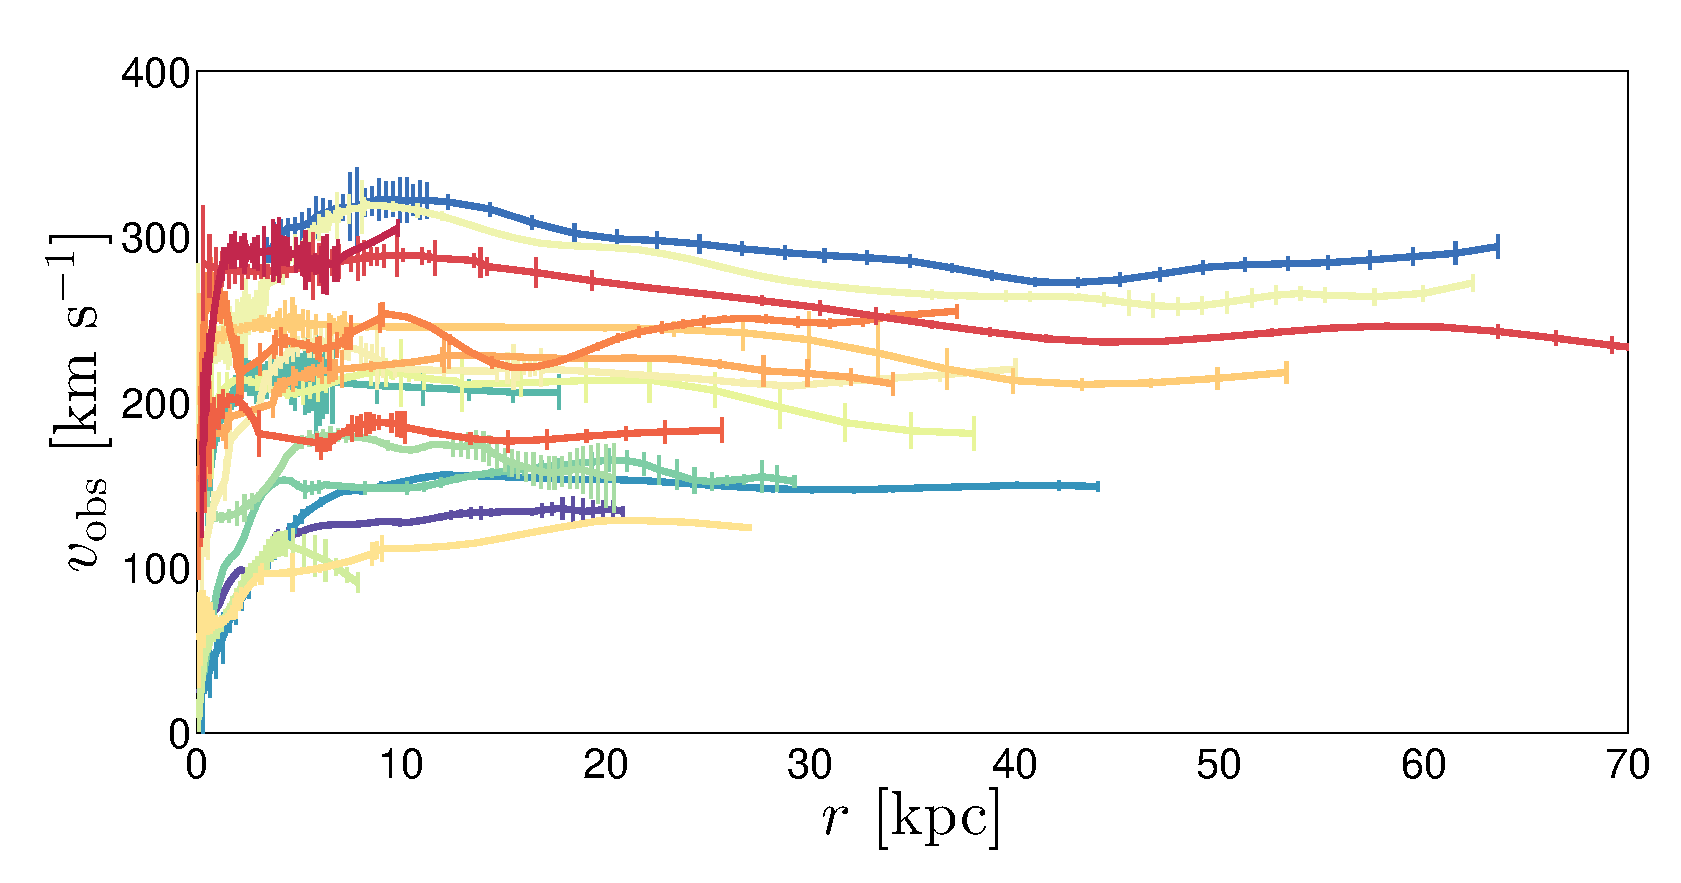
\includegraphics[width=\textwidth]{Figures/galrot.eps}
\caption[SPARC galaxy rotation curves]{Sample of disk galaxy rotation curves from SPARC. The rotation curves are shown as observed speed $v_{\rm obs}$, as a function of radius $r$. Despite the galaxy-to-galaxy differences there is consistent flattening at large $r$, contrary to the Keplerian prediction.}\label{fig:galrot}
\end{center}
\end{figure}

\subsection{Galaxy clusters}\label{sec:intro_galclusters}
Galaxy clusters contain 100~-~1000 galaxies of varied size and are the largest gravitationally bound structures in the Universe. They were also the first objects to have observations indicate the need for dark matter. Zwicky's 1933 observation of the Coma cluster showed a discrepancy of a factor of a few hundred between the luminous mass and the gravitational mass implied by the virial theorem~\cite{Zwicky:1933gu}. Since these early observations, many more sensitive probes of galaxy cluster masses have been developed. Gravitational lensing techniques involving the analysis of distorted images of distant galaxies due to the deep potential of clusters can be used as an independent measure of the total gravitational mass~\cite{Bartelmann:1999yn,Applegate:2012kr,Applegate:2015kua}. Strong gravitational lenses can also be used to weigh the masses of individual galaxies~\cite{Oguri:2013mxl}. Complementary to lensing, X-ray bremsstrahlung emission from the hot electron plasma (which typically comprises the majority of the mass of the baryonic component\footnote{We make use of the convention in cosmology to refer to all hadronic and leptonic matter as `baryons'.}) can be used to construct temperature profiles and subsequently an independent estimate of a cluster mass~\cite{Vikhlinin:2005mp,Ettori:2013tka,Ettori:2014wea,Tchernin:2015jda}. A combination of these observations with more sophisticated mass modelling and virial estimates~\cite{Carlberg:1995aq} together provide another overwhelming set of evidence for dark matter~\cite{Bryan:1997dn}. Furthermore there are individual cases of galaxy cluster collisions~\cite{Clowe:2006eq,Bradac:2008eu,Dawson:2011kf,Harvey:2015hha} (such as the archetype ``Bullet Cluster'' 1E0657-56~\cite{Markevitch:2003at}) which appear to show a striking separation between the luminous matter and a non-interacting dark component. Because galaxy clusters are the largest structures in the Universe it is not unreasonable to assume that they will be a good indicator of the contents of the Universe~\cite{Freedman:1997vk}. The evidence for dark matter from galaxy clusters and the evidence from rotation curves rely on independent measurements and probe length and mass scales many orders of magnitude apart, so when combined make a persuasive argument.

\subsection{Cosmology}\label{sec:intro_cosmology}
Galaxies aside, arguably the most compelling evidence for dark matter arrived with the advent of precision cosmology. The harbingers of this new era were satellites such as WMAP~\cite{Spergel:2003cb,Spergel:2006hy,Komatsu:2010fb} and subsequently Planck~\cite{Ade:2013zuv,Ade:2015xua} with measurements of the temperature anisotropies in the cosmic microwave background (CMB). Together with the rapidly expanding catalogues of large scale structure (LSS) from surveys such as SDSS~\cite{York:2000gk}, 2dF~\cite{Cole:2005sx}, DES~\cite{Abbott:2005bi} and CFHTLenS~\cite{Heymans:2012gg}, we now have an incredibly detailed view of the contents and evolution of the Universe on the largest scales and over the longest times.

The CMB is the ``first light'' of the Big Bang. It is a snapshot of the time of last scattering, when the Universe was around 380,000 years old. The release of photons occured when nuclei and electrons combined to form neutral atoms, making the Universe transparent for the first time. The spectrum of photons from the CMB form the most precise black body spectrum ever observed in nature with a temperature of 2.725~K~\cite{Fixsen:2009ug}. Despite this it has vitally important fluctuations in temperature across the sky with amplitudes $<~10^{-5}$~\cite{Smoot:1992td}, that may have originated from quantum fluctuations in a fundamental field driving a period of rapid inflated expansion~\cite{Guth:1980zm}. The gravitational collapse of the dark matter found in the subsequent overdensities and the infall of baryons into their potential wells, ultimately form the galaxies and clusters we see in the present day Universe. As well as temperature anisotropies across the sky the CMB photons have anisotropies in their polarisation, the distribution of which is also influenced by processes in the early and late Universe. Of particular note is the primordial B-mode polarisation which are a characteristic of gravitational waves produced generically in models of inflation~\cite{Ade:2014xna,Ade:2015lrj}.

Decomposing the distribution of CMB fluctuations as a function of angular scale, one can construct a power spectrum containing a series of peaks which encode the geometry, contents, and evolution of the early stages of the Universe. The peaks are formed due to acoustic oscillations in the photon-baryon fluid as the gravitational collapse of matter is resisted by the outward radiation pressure. Once this collapse has allowed structure to form, the CMB is imprinted upon again with an assortment of secondary anisotropies. As the CMB photons travel towards us they are blue- and redshifted by falling into and out of gravitational potentials (the Sachs-Wolfe effect~\cite{Giannantonio:2008zi}). The potential wells of galaxy clusters can also distort temperature and polarisation anisotropies on certain scales due to gravitational lensing. The spectrum of the CMB itself is also modified on very small angular scales by the Sunyaev-Zel'dovich (SZ) effect in galaxy clusters when photons are inverse Compton scattered by the hot electron plasma of the intra-cluster medium~\cite{Komatsu:2002wc}. Since the SZ effect is independent of redshift it can be used to count clusters out to large distances. The oscillatory behaviour of the photon-baryon fluid is also inscribed onto the power spectrum of the distribution of matter, meaning catalogues of large scale structure from galaxy surveys contain a valuable distance scale on the later Universe. In the context of LSS these are referred to as baryon acoustic oscillations (BAOs).

The most recent measurement of the angular power spectrum of the temperature and polarisation anisotropies of the CMB by Planck can be fit to good agreement by one of the simplest cosmological models in which the Universe is dominated by a cosmological constant $\Lambda$ and cold dark matter (CDM): the $\Lambda$CDM model. The cosmological constant is a uniform contribution to the energy density of the vacuum and is the simplest explanation for the apparent late time accelerated expansion of the Universe as indicated by the redshifts of type-1a supernovae~\cite{Riess:1998cb,Perlmutter:1998hx,Perlmutter:1998np}. 

To quantify the contents of the Universe we refer to the density of cosmological species as a fraction of the critical density (the density required for a flat Universe) $\Omega_i = \rho_i/\rho_c$, where $\rho_c = 3H_0^2/8\pi G$ in terms of the present day Hubble parameter $H_0$. When combined with complementary measurements from BAOs, weak lensing and type-1a supernovae, the Planck analysis find values of $\Omega_{\rm b} = 0.0486 \pm 0.0010$ and $\Omega_{\rm dm} = 0.2589 \pm 0.0057$ (when $H_0~=~67.74~\pm~0.46\,\,{\rm km\,s}^{-1}\,{\rm Mpc}^{-1}$~\cite{Ade:2015xua}) for the densities of baryons and cold dark matter respectively. In other words 84\% of matter is non-baryonic\footnote{Measurements of the densities of cosmological species are dependent on the square of present day Hubble parameter. Because of historical disagreement between local (e.g. Ref.~\cite{Riess:2016jrr}) and CMB measurements of $H_0$ it is usually expressed as the dimensionless $h~=~H_0/100\,\,{\rm km\,s}^{-1}\,{\rm Mpc}^{-1}$. In some cases we neglect to include $h$ to give an intuitive picture of an $\Omega_i$ as a fraction of the Universe's `energy budget'. In these cases we have inserted the local value mentioned above.}. This leaves the remainder of the energy budget of the Universe, $\Omega_\Lambda~\simeq~1-\Omega_{\rm b}~-~\Omega_{\rm dm}$ as the cosmological constant (since the Universe indeed appears to be flat~\cite{Komatsu:2010fb}, we have $\sum \Omega_i = 1$).

The need for dark matter is indicated from cosmological data alone simply due to the fact that baryonic density fraction is smaller than the total matter density fraction. The argument is made even more compelling still once these measurements are combined with an independent calculation known as Big Bang Nucleosynthesis (BBN). The calculation involves a solution to equations which govern the creation of the lightest nuclides ($^2$H, $^3$He, $^4$He and $^7$Li) during the first few minutes after the Big Bang and then matching the calculated abundances with observations~\cite{Alpher:1948ve,Yang:1983gn,Walker:1991ap}. Ultimately it is the ratio of baryons-to-photons ($n_b/n_\gamma~\sim~10^{-10}$) that dictates the resulting abundances and we can use this to infer the baryon density independently~\cite{Fields:2006ga,Fields:2014uja}. Updated BBN calculations that include uncertainties in measured abundances and nuclear rates set a range for the baryon density of $\Omega_{\rm b} = 0.048 - 0.052$~\cite{Ichimasa:2014fea} which is consistent with Planck and, crucially, smaller than the total matter density. The success of the standard BBN calculation - particularly the prediction of the abundance of deuterium - seems to disfavour the need for anything more exotic than CDM. Although the long-standing overestimate of the abundance of $^7$Li known as the `lithium problem' could be a hint towards the need for new physics (e.g. Ref.~\cite{Fields:2011zzb}).

\subsection{Simulations}
In the $\Lambda$CDM model while the cosmological constant is the dominant influence on the evolution of the Universe in the present day, we attribute the initial formation and growth of structure to cold dark matter. Baryons alone could not have formed large scale structure on the scales we see, or in a short enough time~\cite{Blumenthal:1984bp}. The processes through which overdensities collapse and form the distribution of structure is now well understood due to the success of large N-body simulations. In 2005, the Millenium simulation~\cite{Springel:2005nw}, the largest at the time, modelled the gravitational interactions of 2160$^3$ particles to track the evolution and growth of initial density perturbations in the early Universe. The results of these simulations, the network of sheets, links and filaments known as the cosmic web, show excellent agreement with the distribution of matter in wide surveys of galaxy redshifts~\cite{Cole:2005sx}.

Since then, advances in technology have allowed great improvements in the efficiency and accuracy of simulations on small scales and now include a variety of new physical processes involved with the inclusion of baryons. The most sophisticated projects such as the APOSTLE~\cite{Sawala:2015cdf,Oman:2016zjn} and EAGLE~\cite{Schaye:2014tpa} simulations, which trace the evolution of a small number of low-redshift Milky Way-like galaxies, are enriched with baryonic effects such as supernova feedback, stellar evolution and the physics of atomic and molecular gas. Hydrodynamic simulations can now self-consistently include the back reaction of baryons on dark matter and can trace the evolution of matter both inside galaxies and in the intergalactic medium. Importantly these simulations can have the level of baryonic interaction calibrated to match known relationships between different observables, such as the stellar or black hole masses of galaxies.

Simulations have now largely confirmed the central prediction of the cold dark matter paradigm: the assembly of structure by hierarchical merging of smaller halos to form larger ones~\cite{White:1977jf,Davis:1985rj,Kauffmann:1993jn,Kauffmann:1995gh}. Only a small number of notable problems remain (particularly in dark matter only N-body simulations), which relate to the internal structure of dark matter halos and subhalos. For instance the largest subhalos in simulations seem to be too dense to explain why the Milky Way's own largest satellites are so dim, so-called the `too big to fail' problem~\cite{BoylanKolchin:2011de}. There are also discrepancies between the cuspiness of the central density profiles of simulated satellite galaxies compared with the cored nature of their observed counterparts (the `core-cusp' problem~\cite{Moore:1994yx,Navarro:1996bv}). Lastly, the true abundance of satellite galaxies appears to be much smaller than predicted in simulations (the `missing satellite' problem~\cite{Klypin:1999uc}). Many of these problems have been alleviated either with a more careful treatment of baryonic feedback~\cite{Pontzen:2011ty,Governato:2012fa} or through more thorough and sensitive searches for fainter dwarf satellite galaxies~\cite{Simon:2007dq}. Alternatively they may be suggesting a need for the modification of $\Lambda$CDM as we will discuss shortly.

% Required properties of cdm

\section{Candidates for dark matter}\label{sec:intro_candidates}
The myriad pieces of evidence from astronomy and cosmology argue one of the best cases for particle physics outside of the standard model (SM). Devising sensible theoretical extensions to explain dark matter is an exciting challenge, but also a frustrated one given the success of the SM in explaining with remarkable accuracy the vast majority of experimental results. Dark matter especially presents a novel set of challenges as its known properties, though few in number, are supported by a wealth of precise observational evidence. In this Section we discuss some possible candidates for dark matter from a variety of different theoretical origins.

\subsection{Non-particle dark matter}\label{sec:intro_nonparticle}
While it is enticing to view the evidence for dark matter as an indication of new particles, we must first be sure that it cannot be explained with what we already know to exist. It was once believed that the missing mass in galaxies could consist of small dark objects formed through already understood astrophysical processes. If these were large and abundant enough to constitute a decent proportion of the halo but small enough and with low enough luminosity to evade detection, then they would be a natural solution to the missing mass problem. The umbrella term became `massive compact halo objects' (MACHOs) and would consist of a large, otherwise unaccounted for collection of faint stellar remnants, brown dwarfs, planets and other rocky debris. Now MACHOs have been ruled out as any sizable fraction of dark matter ~\cite{Freese:1999ge} by the absence of the microlensing events they would cause as they pass along lines of sight to nearby stars ~\cite{Tisserand:2006zx, Alcock:2000ph}. White dwarfs can also be independently excluded as a significant contribution to MACHOs because their formation in the required amounts would induce a much more chemically enriched intergalactic medium than observed~\cite{Fields:1999ar}. 

Another possibility is that dark matter is in the form of primordial black holes (PBHs) which are the relics of collapsed early Universe density perturbations~\cite{Carr:1974nx}. PBHs forming before BBN would be non-baryonic and an excellent dark matter candidate because in principle no new physics would need to be invoked to explain their existence\footnote{Unfortunately, based on existing constraints it is often not possible to produce enough PBH dark matter without some new physical mechanism involved with their formation~\cite{Carr:2016drx}.}. The abundance and masses of primordial black holes have been tightly constrained with microlensing searches~\cite{Tisserand:2006zx}, the dynamical heating dwarf galaxies~\cite{Brandt:2016aco}, the disruption of wide binary systems~\cite{Chaname:2003fn}, and the effect of Hawking radiation or accretion X-rays on the CMB~\cite{Clark:2016nst,Ricotti:2007au}. The attention on PBHs was reinvigorated in 2016 when the gravitational wave interferometry experiment LIGO made the first detection of gravitational waves due to the collision of two $\sim$10~$M_\odot$ black holes~\cite{Abbott:2016blz,Abbott:2016nmj}. The improbability of such a large event, based on existing star formation models, has drawn many to reconsider the possibility of PBHs in the same mass range~\cite{Bird:2016dcv,Sasaki:2016jop}. Despite the fact that $1 - 10^3\,M_\odot$ PBHs were excluded as a majority dark matter candidate by microlensing and dwarf galaxy dynamics, it was argued that the delta function mass spectrum assumed in placing these constraints was not appropriate for representing a population of PBHs left over from inflationary density perturbations~\cite{Kuhnel:2017pwq}. However a subsequent revision of these limits finds that no extended mass function can consistently explain both microlensing and dynamical constraints~\cite{Green:2016xgy}. It is hoped that upcoming observations of strongly lensed fast radio bursts will tightly constrain PBHs as a dark matter candidate in this mass range~\cite{Munoz:2016tmg}.

There have been long-standing efforts to attempt to explain the astrophysical evidence for dark matter with modifications to gravity. The best known example is Milgrom's Modified Newtonian Dynamics (MOND) where for very small accelerations the usual law of Newtonian gravitational attraction no longer applies~\cite{Milgrom:1983pn,Milgrom:1983ca,Milgrom:1983zz}. MOND has been successful in explaining the rotation curves of galaxies as it was designed to do~\cite{Sanders:1996ua}, but it has also seen recent success in explaining relationships between the baryonic and gravitational masses of galaxies. Empirical correlations such as the baryonic Tully-Fisher~\cite{McGaugh:2000sr,McGaugh:2011ac} and radial acceleration~\cite{McGaugh:2004aw,Lelli:2017vgz,McGaugh:2016leg} relationships are naturally explained in the context of MOND, and these recent results are in accordance with the initial predictions of Milgrom~\cite{Milgrom:2016uye}. It has also been shown that other modifications to gravity~\cite{Moffat:2016ikl} including screened fifth forces~\cite{Burrage:2016yjm} can recover the relationships. Such laws would not naively be expected from CDM, however it as also been argued that the effects of baryonic physics and the subsequent back reaction of dark matter during the formation of galactic disks explains why a connection between baryonic and gravitational masses occurs~\cite{Navarro:2016bfs,Sales:2016dmm}.

The difficulty in constructing a purely gravitational explanation for dark matter is that as well as explaining observations on a galaxy-to-galaxy basis, it is essential that MOND can emerge from a fully relativistic theory of gravity. In addition to simply recovering the remarkable successes of general relativity on Solar System scales, we also require a formalism for calculating cosmological perturbations and gravitational lensing. Bekenstein's Tensor-vector-scalar gravity (TeVeS) is a covariant generalisation that reproduces MOND in the weak field limit~\cite{Bekenstein:2004ne}. MOND and TeVeS are generally disfavoured as an explanation for dark matter principally because of limited success in explaining the diverse catalogue of evidence. Galaxy rotation curves are a simple testbed but a modified gravity must also self-consistently explain lensing data, the distribution of matter in colliding galaxy clusters and the power spectrum of large scale structure~\cite{Ferreras:2012fg,Mavromatos:2009xh,Ferreras:2009rv}. Most damningly however, the evidence for $\Omega_{\rm b} < \Omega_{\rm m}$ indicated by the CMB and BBN is particularly difficult to explain from this perspective when compared to $\Lambda$CDM~\cite{Slosar:2005fg}. 

% Anne disagrees about the core-cusp problem

\subsection{Neutrinos}\label{sec:intro_neutrinos}
As the evidence for dark matter was beginning to emerge, many believed that the unexplained extra mass in the Universe might be accounted for with neutrinos, the properties of which were (and still remain) largely mysterious. Neutrinos naively fit the bill in that they possess a small mass and certainly interact rarely enough for them to have evaded detection. We now believe however that neutrinos cannot make up even a significant amount of the dark matter for two main reasons. 

The first argument involves their cosmological abundance. Neutrinos were produced in the early Universe in thermal and chemical equilibrium with a bath of other standard model particles. As the Universe expands and cools the rate of interactions producing and destroying neutrinos slows. Eventually below a certain temperature the equilibrium of neutrino production cannot be maintained and the neutrinos will `freeze-out' with a certain abundance called the relic density. Neutrinos freeze-out at a temperature of $T \sim \mathcal{O}(1\,{\rm MeV})$ when the interaction rate $\Gamma_\nu(T)$ falls below the expansion rate given by the hubble parameter $H(T)$. The rate is proportional to the thermally averaged cross section $\langle \sigma_\nu v \rangle$ on the order the Fermi constant, $\sigma_\nu \sim G_F^2$. After freeze-out neutrinos essentially interact only gravitationally so the final relic density is given by the sum of the neutrino masses~\cite{Lesgourgues:2006nd},
\begin{equation}\label{eq:nudensity}
 \Omega_\nu h^2 = \frac{\sum_{i=1}^3 m_{\nu_i}}{93.14\,{\rm eV}} \, .
\end{equation}
Solar and atmospheric neutrino oscillation experiments can measure mass differences between two neutrino mass states from which it can be inferred that the sum of the neutrino masses must be larger than $\sum m_{\nu_i} > 0.06$~eV~\cite{GonzalezGarcia:2012sz}. An upper bound can also be estimated with tritium $\beta$-decay experiments to be around $\sim$6~eV~\cite{Drexlin:2013lha,Lesgourgues:2014zoa}. Hence the density of neutrinos in the Universe must be less than $\Omega_\nu \lesssim 0.14$ and are unlikely to be able to account for dark matter.

In fact, cosmological data has been used to set an even tighter upper limit on the sum of the neutrino masses. The constraint is made by extending the minimal $\Lambda$CDM model by promoting $\sum m_{\nu_i}$ to a seventh free parameter\footnote{Interestingly, cosmological bounds on neutrinos are becoming so stringent that they will soon be able distinguish between the normal and inverted ordering of their mass states~\cite{DeBernardis:2009di}.}. The most recent bound from a combination of Planck polarisation and temperature anisotropies with BAO data is $\sum m_{\nu_i} < 0.151$~eV~\cite{Vagnozzi:2017ovm}. Note that the fit assumes a population of massive neutrinos {\it in addition} to cold dark matter. These early Universe neutrinos make up a background of relics with a temperature slightly lower than the CMB and a present day density of around 300 cm$^{-3}$. Unfortunately with redshifted energies around $10^{-4}$~eV the detection prospects are slim~\cite{Betts:2013uya}.
 
The second and now most critical argument disfavouring neutrinos as a dark matter candidate is from the perspective of the distribution of large scale structure. As mentioned in the previous section cosmological data appears to be well fit by a Universe containing $\Lambda$ and {\it cold} dark matter. The distinction between hot versus cold dark matter is in whether the dark matter is produced relativistically or not. Neutrinos were widely discussed as a hot dark matter (HDM) candidate~\cite{Pogosian:1994ns} but were eventually excluded due to their disastrous effect on structure formation. The central problem is that the growth of structure from initial density perturbations is washed out below a certain scale due to the thermal motions of particles. This scale is set by the typical comoving distance over which particles travel over the age of the Universe and results in a cutoff in the power spectrum of matter at large wavenumbers~\cite{Frenk:2012ph}. This so-called free streaming length decreases with the mass of the particle $\lambda~\propto ~m^{-1}$ and for neutrinos (or any HDM) this cuts off structure below the size of a galaxy cluster. In a Universe in which neutrinos are dark matter the formation of galaxy sized halos is impossible. As such the cold dark matter paradigm - permitting structures much smaller than observed dwarf galaxies - has become the preferred cosmology.

It is worth briefly mentioning the intermediate case known as warm dark matter (WDM), for masses $m \sim 2$ keV when the free streaming length is roughly on the scale of a dwarf galaxy. There are some hints this may solve problems in comparisons between simulations and the observed structure of dark matter halos. WDM has been shown in the past to ease problems with the cores of dwarf galaxies~\cite{Boyanovsky:2007ay} or the `too big to fail' problem~\cite{Lovell:2016nkp}. Candidates for WDM are also theoretically motivated. An example, sterile neutrinos, are a heavier fourth species of neutrino that undergo oscillations but have no electroweak interactions~\cite{Dodelson:1993je,Kusenko:2006wa}. Sterile neutrinos appear in many extensions of the standard model such as seesaw mechanisms to explain the masses of the three `active' neutrinos~\cite{Abazajian:2012ys} and there have been suggestions that some experimental anomalies cannot be explained by the mixing of only three neutrinos~\cite{Aguilar-Arevalo:2013pmq,Aguilar:2001ty,Mention:2011rk,Adamson:2016jku}. Sterile neutrinos have also been shown to slightly alleviate tensions between CMB and LSS data~\cite{Battye:2013xqa,Battye:2014qga} and their decay has been invoked in explanations of unidentified X-ray emission lines~\cite{Boyarsky:2014jta,Bulbul:2014sua}. However it remains to be seen if these problems can all be resolved consistently with the same sterile neutrino or if there is a mechanism to produce them in the right amounts~\cite{Shakya:2015xnx}. Furthermore many of these problems can be explained by other means. 

\subsection{WIMPs}\label{sec:intro_WIMPs}
Cosmological data dictates that dark matter must be produced cold and collisionless with a relic density of $\Omega_{\rm dm} h^2 =  0.1188 \pm 0.0010$~\cite{Ade:2015xua}. We also know that it must be stable, at least over the time taken to affect the CMB and still be present in galaxy halos today. But given that we are yet without indication of the precise particle nature of dark matter we know that it must have interactions small enough with the remaining three forces for it to have not caused too much disruption to structure formation or otherwise unexplained excesses in radiation. For instance, dark matter with any significant electromagnetic charge ($>10^{-6}e$ for a 1 GeV mass dark matter particle for example) would heavily disrupt the formation of the acoustic peaks of the CMB~\cite{McDermott:2010pa}. Any other sizable interactions for instance via the strong force or to any electrically neutral particle would provide an additional mode of energy transfer between baryons and dark matter and and would generally slow galaxy formation. What remains allowed however is a general class of dark matter candidate: weakly interacting massive particles (WIMPs). WIMPs are heavy, stable, weakly coupled particles that are assumed to self annihilate. The WIMP dark matter hypothesis is famously motivated with an argument known as the `WIMP miracle'~\cite{Wolfram:1978gp,Srednicki:1988ce,Scherrer:1985zt,Gondolo:1990dk}. 

As we described previously, particles that are in thermal equilibrium of creation and annihilation during some early epoch undergo freeze-out. This occurs when the expansion and cooling of the Universe dilutes the particles to a density at which they are being produced at a rate slower than the expansion rate $H$. The interaction rate is given by the thermally averaged annihilation cross section $\Gamma = n_\chi \langle \sigma_{\rm ann} v \rangle$. The number density of particles in equilibrium with $g$ internal degrees of freedom can be defined~\cite{Jungman:1995df},
\begin{equation}
 n_\chi(t) = \frac{g}{(2\pi)^3} \int \textrm{d}^3 p \, f(E,t) \, ,
\end{equation}
where $p$ is momentum and $f(E,t)$ is the time dependent phase space distribution determined by the spin statistics of the particle i.e. bosonic or fermionic. As the Universe expands the evolution of the number density will evolve according to the Boltzmann equation,
\begin{equation}\label{eq:boltzmann}
 \frac{\textrm{d}n_\chi}{\textrm{d}t} + 3 H n_\chi = -\langle \sigma_{\rm ann} v \rangle \left[ n_\chi^2 - (n_\chi^{\rm eq})^2\right] .
\end{equation}
In which $n^{\rm eq}_\chi$ is the equilibrium number density of dark matter particles which follows a Maxwell-Boltzmann distribution,
\begin{equation}
n^{\rm eq}_\chi \sim \left\{
\begin{array}{llrr}
T^3 &	\ \text{for $T \gg m_\chi$\,}  \\
(m_\chi T)^{3/2} \exp(-m_\chi/T)	& 	\ \text{for $T \ll m_\chi$\,,} 
\end{array}\right.
\end{equation}
depending on the temperature $T$ relative to the WIMP mass $m_\chi$. We see then from Eq.~(\ref{eq:boltzmann}) that for temperatures where the reaction rate is larger than the Hubble rate $\Gamma> H$, the number density is maintained at $n_\chi^{\rm eq}$. However as the Universe inevitably expands, the temperature will drop and for low $T$ the number density becomes Boltzmann suppressed by the exponential factor. Eventually the Hubble expansion rate which falls with temperature more slowly, ($H \propto T^2$ during radiation domination for example) will eventually exceed $\Gamma$. When it does the average time per interaction becomes longer than the age of the Universe and WIMP annihilation and creation can no longer maintain equilibrium. At this point the WIMPs chemically decouple from the thermal bath and their number freezes out leaving a final population of dark matter relics for the remainder of cosmic time. The temperature of freeze-out $T_f$ can be found by setting $\Gamma(T_f) \sim H(T_f)$. The relic density then follows after solving the Boltzmann equation at the present day, with initial conditions $n_\chi^{\rm eq}(T_f)$ and the removal of the collisional term (i.e. Hubble dilution $\textrm{d}n_\chi/\textrm{d}t = -3 H n_\chi$). The final density parameter in terms of the thermally averaged annihilation cross section is~\cite{Wolfram:1978gp,Srednicki:1988ce,Scherrer:1985zt,Gondolo:1990dk}
\begin{equation}\label{eq:relicdensity}
 \Omega_{\rm dm} h^2 \simeq 0.1 \left(\frac{3 \times 10^{-26}\,\,\textrm{cm}^3\,\textrm{s}^{-1}}{\langle \sigma_{\rm ann} v\rangle}\right) \, .
\end{equation}
Expressing $\Omega_{\rm dm}$ in this form shows that the observed relic density of dark matter points to a canonical value for the thermally averaged cross section around the weak scale. This argument is rather general and in practice many additional physical effects must be taken into account in accurate calculations of the relic density, for instance we have neglected the dependence on the WIMP mass and variation in the number of degrees of freedom~\cite{Steigman:2012nb}. However the basic argument holds and provides compelling motivation for candidate particles interacting with the standard model via the weak sector. The `miraculous' element of the WIMP miracle is that the argument points to particles which are simultaneously one of the only generic classes consistent with observation. The hypothesis also implies its own testability using three independent and complementary detection strategies that we discuss in Sec.~\ref{sec:intro_detection}.

Secondary, but rather crucial motivation for WIMPs originates from their natural appearance in many beyond the standard model theoretical frameworks, most notably that of supersymmetry (SUSY)~\cite{Jungman:1995df}. Supersymmetry is a principle which may be added to the fundamental construction of the SM to posit a symmetry between matter and forces, i.e. between fermions and bosons. It was realised in the 1970s that the normal symmetries of the S-matrix of quantum field theories (Lorentz boosts, rotations and translations, as well as internal symmetries) could be extended with the inclusion of generators that convert between bosonic and fermionic states~\cite{Gervais:1971ji,Akulov:1974xz,Wess:1974tw}. A theory that obeys supersymmetry has bosonic and fermionic states paired with identical mass and quantum numbers except for a difference in spin of $1/2$~\footnote{Superpartners to standard model fermions are bosons called sfermions with the prefix `s'. Superpartners to the standard model gauge bosons are fermions called gauginos with the suffix `ino'.}. Since we cannot pair up the standard model like this and no evidence has been found for any new particles, if supersymmetry is a symmetry of nature it must be broken meaning the masses of the superpartner particles exist beyond the TeV scale. Broken or otherwise, supersymmetric models are important solutions to a number of existing problems, most notably the ``hierarchy problem".

It is well known that the calculation of the Higgs mass is drastically unstable and sensitive to any unknown physics that might exist in the gulf between the electroweak and the Planck scales. The quantum corrections received by the squared Higgs mass from for instance, the heavy quarks, turn out to be large and quadratically sensitive to the ultraviolet cutoff between these two scales used to regularise the loop integrals. This ultraviolet cutoff is the scale at which the standard model ceases to be valid and a good effective theory should desirably be insensitive to it. Unfortunately this scale may be anywhere between a few TeV and the Planck scale $>10^{19}$ GeV. So for the weak scale masses of the Higgs, the W and the Z to be maintained this ends up requiring fine tuning of up to 1 part in 10$^{34}$.  In general SUSY rescues the divergence because the corrections from all the fermionic/bosonic standard model particles are cancelled by their bosonic/fermionic superpartners and the Higgs mass is stabilised.

In many SUSY models, to ensure the stability of the proton the conservation of $R$-parity is enforced. $R$-parity is defined as
\begin{equation}
R = (-1)^{3B+L + 2S}\, ,
\end{equation}
for states with baryon number $B$, lepton number $L$ and spin $S$. This quantum number is +1 for standard model particles and -1 for their superpartners~\cite{Martin:1997ns}. If $R$-parity is conserved then the decays of any SUSY particle must contain odd numbers of other SUSY particles. This means that the lightest supersymmetric particle (LSP) is energetically required to be stable as there are no lighter SUSY particles to which it can decay. Such particles are excellent dark matter candidates, providing further motivation for SUSY. In many models the favoured LSP is the neutralino which is a mixed state consisting of a linear combination of the neutral -inos (the Higgsinos and neutral wino and bino). The lightest neutralino in the simplest realisation of supersymmetry, the minimal supersymmetric standard model (MSSM), has typically a $\sim$100~GeV~-~1~TeV mass~\cite{Jungman:1995df} and is a Majorana fermion so self-annihilates as required.

Other SUSY models such as the next to minimal supersymmetric model, constrained minimal supersymmetric model or minimal supergravity can predict other superpartners for the LSP and may give rise to other dark matter candidates: the gravitino, sneutrinos or axino for example. Moreover, alternative beyond-the-standard-model frameworks such as universal extra dimensions models can predict WIMP candidates~\cite{Hooper:2007qk}. For the remainder of this thesis however we consider only the generic WIMP and remain agnostic with regards to its deeper origin. 
% NEED REFS FOR ALL THESE MODELS

\subsection{Axions and axion-like particles}\label{sec:intro_axions}
Axions are light pseudoscalar particles that appear in the solution of Peccei and Quinn~\cite{Peccei:1977hh, Kim:2008hd} to explain the unnatural absence of CP-violation in quantum chromodynamics (QCD)\footnote{CP denotes the combination of charge conjugation and parity transformations which can either be conserved or violated in a theory.}. This strong CP problem as it is known arises because of an apparent need to fine tune a CP violating phase $\bar{\theta}$ to a value less than $10^{-14}$~\cite{Baker:2006ts} where in principle it could take any value from 0 to $2\pi$ with seemingly no anthropic preference. The Peccei-Quinn solution is to promote this phase to a field which is driven to 0 dynamically after the spontaneous breaking of a new U(1) symmetry. The mechanism predicts the existence of a new light pseudoscalar which was called the axion~\cite{Wilczek:1977pj,Weinberg:1977ma}\footnote{The axion was named after an American brand of laundry detergent by Wilczek since it was said to ``clean up" a problem with an ``axial'' current; narrowly missing out on the name ``Higglet'' as suggested by Weinberg~\cite{Wilczek:quantamag}.}. There are various models for how this symmetry breaking takes place that predict particular relationships between the axion mass and the strength of its couplings to the SM. The axion predicted in these models is referred to as the `QCD axion'. More recently, motivation from the landscape of axion-like particles (ALPs) appearing in string theory~\cite{Svrcek:2006yi,Arvanitaki:2009fg,Cicoli:2012sz} has inspired the generalisation of the QCD axion to light pseudoscalars originating outside of the original Peccei-Quinn solution. Such ALPs share phenomenology with the axion but can cover an extremely wide range of masses and couplings~\cite{Arias:2012az}.

Axions and ALPs are attractive cold dark matter candidates and it has been shown that they can be produced in the early Universe through a variety of non-thermal mechanisms such as vacuum misalignment or via the decay of topological defects~\cite{Davis:1986xc,Hiramatsu:2012gg} in ways that are consistent with the known cosmological abundance and phenomenology of CDM~\cite{Ipser:1983mw,Wantz:2009it,Marsh:2015xka}. Axions can be detected thanks to a coupling to electromagnetism which permits their conversion into photons. Certain mass and coupling ranges for ALPs can be ruled out with observations of astrophysical environments expected to produce them in significant quantites e.g. white dwarfs~\cite{Raffelt:1985nj,Isern:2008nt}, neutron stars~\cite{Berenji:2016jji}, red giants~\cite{Raffelt:1999tx} and supernovae~\cite{Burrows:1988ah,Mayle:1987as}. Axions may also be observable in the lab as we discuss in Sec.~\ref{sec:intro_axionexpts}.

\section{Detecting dark matter}\label{sec:intro_detection}
Despite the quantity of gravitationally based evidence, it is clear that the probes of dark matter that we have discussed so far are not sufficient to learn more about its particle nature. In this section we briefly summarise how dark matter may be detected in the future. WIMPs in particular have three principal detection strategies illustrated in Fig.~\ref{fig:detection-diag}. These are {\color{green}{direct detection}} in which WIMPs scatter off standard model targets, {\color{blue}{indirect detection}} in which WIMPs annihilate into standard model particles, and {\color{red}{production}} in colliders. We also discuss experimental searches for axions.

\begin{figure}[t]
\begin{center}
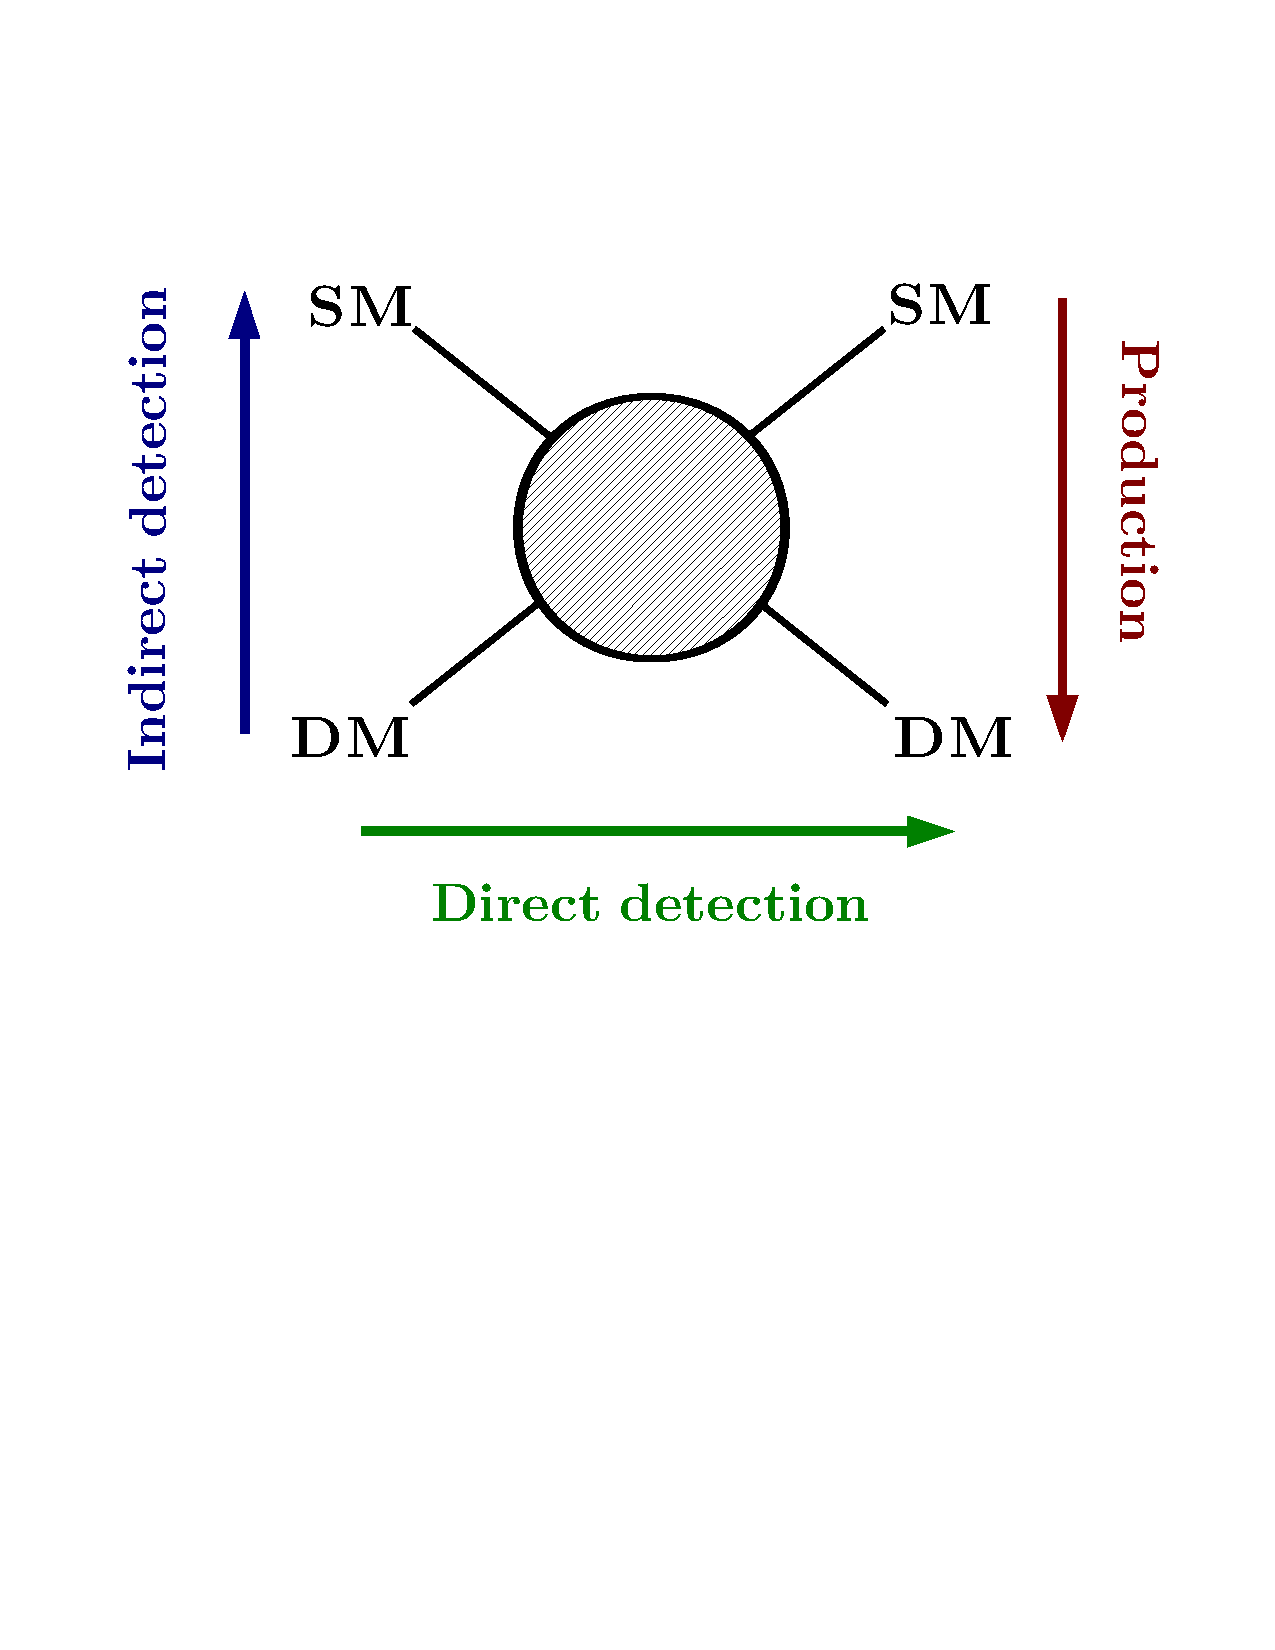
\includegraphics[width=0.7\textwidth,trim = 20mm 120mm 20mm 40mm,clip]{Figures/detection-diag.pdf}
\caption[Three strategies for detecting dark matter]{Diagram of the three principal strategies for detecting dark matter (DM) with standard model (SM) particles.}\label{fig:detection-diag}
\end{center}
\end{figure}

\subsection{Direct detection}\label{sec:intro_direct}
The Solar System is embedded inside a dark matter halo. Estimates from local astronomical data~\cite{Salucci:2010qr,Smith:2011fs,Bovy:2012tw,Garbari:2012ff,Zhang:2012rsb,Bovy:2013raa}, global comparisons with Milky Way mass models~\cite{Weber:2009pt,Catena:2009mf,Iocco:2011jz,Nesti:2013uwa,Sofue:2015xpa,Pato:2015dua} as well as simulations of Milky Way-like galaxies~\cite{Bozorgnia:2016ogo} all predict a non-zero density of dark matter at Earth with a value somewhere in the range $\rho_0 = 0.2 - 0.7$~GeV~cm$^{-3}$. We expect a flux of dark matter particles with speeds $\sim$200~km~s$^{-1}$ on Earth at all times. If WIMPs can scatter off standard model particles it should in principle be possible to see evidence of these interactions by searching for recoiling particles, usually nuclei~\cite{Goodman:1984dc,Drukier:1986tm}. The difficulty in designing a detector to search for these events is that there are a multitude of cosmic and terrestrial sources of background also inducing recoils in the expected keV energy scale. In addition to the steadily increasing physical size of these detectors the last few decades have seen continuous progress in background modelling, reducing energy thresholds and improving signal discrimination; all of which are necessary for pushing down the sensitivity to smaller cross sections and WIMP masses. The current most sensitive direct detection experiments, including LUX~\cite{Akerib:2013tjd}, Xenon100~\cite{Aprile:2011hx} and PandaX~\cite{Tan:2016zwf} have reached spin-independent WIMP-nucleon cross sections around $\sigma \sim  10^{-44}-10^{-46} \, {\rm cm}^2$.

The frontier of direct detection experiments is approaching the ton-scale in mass and near future experiments are expected to reach a sensitivity at which coherent scattering between nuclei and Solar neutrinos will begin to constitute a dominant background~\cite{Monroe:2007xp,Strigari:2009bq,Gutlein:2010tq,Billard:2013qya}. It is predicted that one of the upcoming ton-scale xenon experiments, LZ~\cite{Akerib:2015cja} or Xenon1T~\cite{Aprile:2015uzo}, will make the first measurement of coherent neutrino-nucleus scattering (CNS) due to $^8$B Solar neutrinos\footnote{CNS remains an unmeasured interaction of the standard model, though its cross section has been calculated~\cite{Freedman:1973yd}.}. Since they are impossible to shield, neutrinos are the ultimate background to direct detection. Because of the similarity between WIMP and neutrino recoil energy spectra in direct detection experiments, the large uncertainty in our knowledge of the neutrino flux imposes a lower limit on the discoverable WIMP-nucleon cross section called the neutrino floor~\cite{Billard:2013qya,Ruppin:2014bra,Davis:2014ama,Grothaus:2014hja,O'Hare:2015mda,OHare:2016pjy}.

It may be possible to distinguish neutrinos from WIMPs with the use of smoking gun Galactic dark matter signals. As well as measuring the energy of recoiling nuclei, direct detection experiments could in principle exploit time and direction dependencies. Due to the relative motion of the Earth and Sun with respect to the (largely non-rotating) dark matter halo, the peak flux of WIMPs should point back towards the constellation of Cygnus~\cite{Spergel:1999mh}. As the Earth revolves around the Sun we move with respect to this flux, thus annually modulating the recoil spectrum~\cite{Drukier:1986tm}. By the same argument there is also a very small daily modulation due to the rotation of the Earth~\cite{Bozorgnia:2011tk}. 

% evidence for non-rotating halo?

WIMP direct detection is the subject of Chapters~\ref{chapter:direct}-\ref{chapter:nufloor}. We begin with a detailed theoretical introduction and discussion of the experimental status in Chapter~\ref{chapter:direct}.

\subsection{Indirect detection}\label{sec:intro_indirect}
The annihilation of WIMPs was described in the context of the relic density calculation in the previous section. If WIMPs cluster in the Universe in regions of sufficiently high density then annihilation events may occur in sizable numbers. If the dark matter particle is heavy enough and its products energetic enough then it may be possible to detect them in a range of space and ground based cosmic ray detectors as well as neutrino telescopes. Detection or non-detection of excesses in for example the gamma ray flux from a region of suspected high dark matter density would provide a measurement or constraint on the annihilation cross section. The WIMP miracle suggests that this should be of the order $\langle \sigma_{\rm ann} v \rangle \sim 3 \times 10^{-26}$~cm$^3$~s$^{-1}$, Eq.~(\ref{eq:relicdensity}). 

The most important considerations for indirect searches are finding regions with large expected rates of annihilation that also have either low or well understood astrophysical emission. The proximity and high density of the Galactic center makes it an attractive place to search. Nearby dwarf spheroidal galaxies are also good targets as they are believed to be dark matter dominated with very low non-thermal gamma ray emission~\cite{Evans:2003sc,Fermi-LAT:2016uux}. A particularly desriable signal is a monoenergetic gamma ray line which could be emitted in certain final states. This would have no alternative standard astrophysical explanation and would be a smoking gun~\cite{Bergstrom:1994mg}, although continuum emission from hadronisation and decay of other products is expected to be larger. Predicting the gamma ray flux from annihilations requires first computing the line of sight integral of the square of the dark matter density towards the target (known as the $J$-factor). Then to extract a potential signal, all astrophysical background and foreground gamma ray emission must be modelled and subtracted. Through the non-observation of MW dwarf spheroidal galaxies, Fermi-LAT currently sets the tightest limits on the annihilation cross section~\cite{Ackermann:2015zua}. Of particular note however, an excess in the central 10$^\circ$ towards the Galactic center~\cite{Goodenough:2009gk,Hooper:2010mq} has had many claims put forward for a dark matter interpretation in the past (e.g. Refs.~\cite{Boehm:2014hva,Cahill-Rowley:2014ora,Cerdeno:2015ega,Caron:2015wda,Fonseca:2015rwa,Karwin:2016tsw}), however these can also be explained astrophysically with emission from a stellar overdensity~\cite{Macias:2016nev}, cosmic ray outbursts~\cite{Cholis:2015dea,Carlson:2016iis} or unresolved millisecond pulsars~\cite{Bartels:2015aea,Lee:2015fea,OLeary:2016cwz} for example. Furthermore, the most recent re-analysis by Fermi~\cite{TheFermi-LAT:2017vmf} has found similar sized excesses in other regions of the Galactic plane where no annihilation signal is expected. Going to larger energies than Fermi, due to the sharply decreasing gamma ray flux, larger effective areas are required. This makes ground based imaging atmospheric Cherenkov telescopes such as MAGIC~\cite{Doro:2017dqn}, HESS~\cite{Abdalla:2016olq}, VERITAS~\cite{Holder:2008ux}, HAWC~\cite{Proper:2015xya} (and in the future the Cherenkov Telescope Array (CTA)~\cite{Hofmann:2017lob}) more suitable.

Neutrino telescopes such as IceCube~\cite{Aartsen:2016pfc}, ANTARES~\cite{Collaboration:2011nsa}, Super-Kamiokande~\cite{Choi:2015ara} (and in the future Hyper-Kamiokande~\cite{Abe:2011ts}, PINGU~\cite{TheIceCube-Gen2:2016cap} and KM3NeT~\cite{Katz:2006wv}) are also useful for indirect searches since neutrinos, like gamma rays, point back towards their source and retain their spectral information. This is not true of charged cosmic rays which would also be produced in annihilations but propagate along complicated paths due to magnetic fields and have their spectrum softened by environmental processes. Antimatter cosmic rays are generally rare events however, so astrophysical backgrounds for positrons and antiprotons are inherently low. The trade off is in mapping the propagation of these particles through the Galaxy~\cite{Moskalenko:1997gh,Delahaye:2008ua,Strong:2004de}. PAMELA~\cite{Adriani:2008zr}, AMS-02~\cite{Aguilar:2013qda} and Fermi-LAT~\cite{FermiLAT:2011ab} have now all confirmed an unexpected rise in the positron to electron ratio from $\sim$10 to $\sim$100 GeV. As with other hints, both dark matter interpretations and astrophysical explanations have been suggested (e.g. Ref.~\cite{Fan:2010yq}). Analyses with antiprotons on the other hand are consistent with background models and currently set the best constraints among cosmic ray searches~\cite{Cuoco:2016eej}. The proposed experiment GAPS~\cite{Hailey:2009fpa} is hoped to be particularly powerful with its ability to detect antideuterons for which the astrophysical background is negligible~\cite{Donato:1999gy}.

\subsection{Colliders}\label{sec:intro_colliders}
WIMPs can be expected to be produced in high energy collisions performed in experiments at the Large Hadron Collider (LHC) such as ATLAS and CMS. Dark matter produced in collisions will not interact with the surrounding medium and are expected to stream out of the detector leaving remaining particles with large missing transverse momenta. Typically these are characteristic mono- signals such as -jets, -W, -Z, or -Higgs. ATLAS~\cite{Aad:2013oja,Aad:2015zva,ATLAS:2012ky,Aaboud:2017dor,Aaboud:2017yvp} and CMS~\cite{Khachatryan:2014rra,Khachatryan:2014rwa,Sirunyan:2017onm,Sirunyan:2017hnk,Sirunyan:2017hci} have both conducted searches for dark matter production in proton-proton collisions with a maximum center of mass energy of 13 TeV. To date there appears to be no evidence in significant conflict with the standard model, but constraints can be made. Ideally we would like these bounds to be expressed in the language of direct or indirect detection; in principle the three strategies should be highly complementary. Thankfully there exist frameworks for searching for general dark matter particles in LHC data. For instance the effective field theory approach (e.g.~\cite{Beltran:2010ww,Goodman:2010yf}) in which the SM-DM production is described as a contact interaction, or `simplified models' (e.g.~\cite{Buchmueller:2014yoa,Garny:2014waa,Liew:2016oon}) which are UV complete but introduce a SM-DM mediator that must also be constrained. However care must be taken as these frameworks carry assumptions which make the direct translation between interpretations of limits on dark matter a non-trivial process. 

Beyond technical considerations, a deeper issue with collider searches is that there is no way to demonstrate that a new particle is cold dark matter. Firstly a particle that streams out of the experiment may not be stable on a cosmological timescale. Secondly and possibly more worryingly is: how do we know if a new `dark' particle is the same as the one found in the Galaxy and beyond? Wheatever the case, any such signal will generate much excitement from the theoretical community\footnote{cf. over 500 arXiv submissions in 2016 about the now diminished diphoton excess at 750~GeV~\cite{750GeV}.} and if confirmed could point the way to more refined direct or indirect searches. 

\subsection{Other interactions}\label{sec:intro_other}
There exist other tests of dark matter interactions that do not fit neatly into this three pronged catagorisation. For example WIMP interactions in stars connect direct and indirect searches and can be used to probe both scattering and annihilation. It was realised some time before the advent of direct detection experiments that the Sun could act as a dark matter detector~\cite{Press:1985ug}. All stars embedded in the halo should sweep up a collection of dark matter particles as they orbit the galaxy. If a dark matter particle scatters off the Sun to a speed below the local escape velocity then it will become gravitationally trapped and left to orbit continuously around the Solar core~\cite{Gould:1987ir,Gould:1991hx}. Over time it is possible that stars could accumulate a high enough density for annihilations to occur. The only products that will be able to escape are neutrinos but these may be detectable on Earth~\cite{Silk:1985ax,Gaisser:1986ha,Srednicki:1986vj}. Observation or non-oberservation of high energy neutrinos from the Sun are another way to make constraints on the annihilation cross section~\cite{Choi:2015ara,Aartsen:2016zhm,Aartsen:2016exj} as well as a complementary way to probe scattering cross sections~\cite{Arina:2013jya,Kavanagh:2014rya}. Beyond our own Sun, in other stars such as white dwarfs annihilations would slow cooling and prolong lifetimes~\cite{Hurst:2014uda}, WIMP `burning' has also been suggested as a source of power for the first stars~\cite{Spolyar:2007qv,Freese:2015mta}.

% should mention cmb constraints 1512.08015 1310.3815	

It is also possible that dark matter interacts in slightly different ways and would not have a detectable signal using the strategies already discussed. For instance it may be that in high densities dark matter undergoes scattering self-interactions rather than annihilations. These observations would not have any direct observable signature in the form of products or decays. Instead self-interaction cross sections must be constrained by searching for distributions of dark matter that cannot be explained in terms of collisionless particles. Some of the small scale problems of N-body simulations, as described earlier, have been used to claim the need for these self interactions. In particular the cuspiness of the cores of simulated dwarf and low surface brightness galaxies could be resolved through heating and expansion via self-interaction~\cite{Spergel:1999mh, Rocha:2012jg, Zavala:2012us, Elbert:2014bma, Vogelsberger:2012ku, Fry:2015rta}, but these claims are in tight competition with constraints from colliding galaxy clusters~\cite{Harvey:2015hha, Randall:2007ph}. 

% what about claims from bullet cluster

\subsection{Axion experiments}\label{sec:intro_axionexpts}
The principal avenue to search for axions and ALPs is through their coupling to electromagnetism. In strong magnetic fields incoming axions can convert into a photon with energy approximately equal to the axion mass~\cite{Sikivie:1983ip}. How best to design an experiment to detect these photons depends on the source of the axions\footnote{We focus here on the coupling to photons but other couplings such as those to nuclei can be probed in nuclear magnetic resonance experiments such as CASPEr~\cite{Budker:2013hfa,Graham:2013gfa}. The axion coupling to electrons can also be constrained in WIMP direct detection experiments~\cite{Aprile:2014eoa,Akerib:2017uem}.}.

{\bf Dark matter axions} streaming in from the Milky Way halo will convert into photons inside magnetic fields in a lab setting although the power they produce will be extremely small. In a resonant magnetic cavity experiment however this axion conversion power is resonantly enhanced which can be achieved if the frequency of the cavity mode matches the axion mass. Since the mass is unknown, an experiment must be designed to scan over a range of resonant frequencies. This is achieved in the flagship `haloscope' ADMX with the use of movable tuning rods placed inside the cavity itself. There also exist alternative techniques with layered dielectric disks~\cite{TheMADMAXWorkingGroup:2016hpc} or dish antennae~\cite{Jaeckel:2015kea,Horns:2012jf}. Since haloscope experiments are the subject of Chapter~\ref{chapter:axions} we delay the full technical discussion until then.

{\bf Solar axions}: The Sun is expected to produce a flux of relativistic axions which can be detected in similar experiments called helioscopes. CAST looks for Solar axions converting into X-rays inside a long cavity pointed at the Sun over long exposure periods during the day~\cite{Zioutas:2004hi}. IAXO is a planned upgrade to CAST and will be able to constrain Solar axion couplings to even smaller values~\cite{Armengaud:2014gea}.

{\bf Laboratory axions}: It may be possible to produce axions in the lab and detect them in light-shining-through-a-wall experiments (LSW)~\cite{VanBibber:1987rq,Redondo:2010dp}. If light from a strong laser is passed through a magnetic field then photons could convert to axions and then back again on either side of an opaque barrier. Currently LSW experiments such as ALPS~\cite{Ehret:2007cm} are not sensitive enough to probe QCD scale axion couplings however the planned upgrade ALPS-II will improve upon the limits of its predecessor by three orders of magnitude~\cite{Bahre:2013ywa}.

It is important to emphasise the epistemological differences between these three experimental strategies. Haloscopes specifically look for dark matter axions/ALPs. Only if, for example ADMX, is successful in its search for axions will it confirm them as a dark matter candidate. If a helioscope or a future LSW experiment detects axions then this may confirm their role in the solution to the strong CP problem, but crucially it will {\it not} confirm them as a dark matter candidate. The other side of the coin to this is that Solar and laboratory experiments do not {\it require} axionic dark matter to detect axions.

\section{Summary}\label{sec:intro_summary}
% check
The success of the dark matter paradigm is borne out of both the quantity and precision of observational evidence but also the variety of that evidence. From sub-galactic scales up to the largest cosmological dataset, the evidence for the presence of dark matter is striking and one of the best arguments for physics beyond the standard model. In this introduction we have outlined two possible candidate classes of particle that are the subject of this thesis: weakly interacting massive particles, and axions. We have discussed their particle physics origin and methods of detection. This thesis will focus on the direct detection of axions and WIMPs, and in particular on future experiments and their potential to study those particles beyond simply identifying them. In particular we are interested in the uncertainty in the phase space structure of dark matter in the local Milky Way. Understanding these astrophysical uncertainties is important in achieving the particle physics goals of dark matter detection. On the other hand, as we will argue, terrestrial dark matter detectors are the only tools suitable for probing this astrophysical dependence.

This thesis is structured as follows. To begin, in Chapter~\ref{chapter:direct} we introduce the foundations for direct detection, deriving the WIMP-nucleus scattering event rate, discussing sources of particle and astrophysics uncertainty and outlining the current and future experimental effort. 

In Chapter~\ref{chapter:directional} we study the discovery reach of dark matter detection with directional sensitivity. We begin with a review of the key theoretical results and summary of the experimental techniques involved before showing how powerful these experiments are for constraining the astrophysical dependence of a dark matter signal. We first detail the particular case of tidal streams before considering general cases and the use of empirical methods for parameterising the velocity distribution.

In Chapter~\ref{chapter:nufloor} we consider future ton-scale experiments which are potentially sensitive to both WIMP and neutrino scattering. We first outline the calculation of the neutrino floor limit to direct detection and then show its dependence on various sources of uncertainty from the neutrino flux and dark matter astrophysical uncertainties. We then study methods of subtracting the neutrino background and potentially circumventing the floor. We briefly comment upon the use of timing information before studying in detail the most powerful method: directional detection. Here we consider a range of experimental uncertainties, in particular lower dimensional readout strategies. 

Finally in Chapter~\ref{chapter:axions} we move to axions. We first review the relevant particle physics motivation and summarise the existing constraints on the axion/ALP mass and coupling to photons. We then explore the potential for future microwave cavity experiments like ADMX to probe the phase space structure of the local dark matter halo. In analogy with the analysis presented in Chapter~\ref{chapter:directional} we devise a statistical technique to extract astrophysical information from simulated haloscope data and apply this to a range of cases including simple halo models, the Solar peculiar velocity, N-body simulation data and finally axion miniclusters.

The appendices contain expanded technical detail for: the laboratory velocity (\ref{app:labvelocity}), spherical statistics (\ref{app:dirstats}), a Monte Carlo scattering simulation (\ref{app:scattering}), the Solar vector (\ref{app:solar}), the profile likelihood ratio test (\ref{app:likelihood}), and expressions for some alternative speed distributions (\ref{app:fv}).